\documentclass[aspectratio=169,9pt]{beamer}
% Beamer layout
\setbeamersize{text margin left=0.4cm, text margin right=0.2cm}

% Math & fonts
\usepackage{amsmath,amssymb}
\usepackage{mathpazo}   % Palatino text + math

% Tables & units
\usepackage{booktabs}
\usepackage{siunitx}

% TikZ (one load, all libs)
\usepackage{tikz}
\usetikzlibrary{arrows.meta,calc,positioning,shapes.geometric,shapes.misc}

% Algorithms
\usepackage{algorithm}
\usepackage[noend]{algpseudocode}
\usepackage{float}

% Media
\usepackage{multimedia}
\usepackage{animate}

% Bibliography
\usepackage{natbib}

\tikzset{
  >={Stealth},
  proc/.style = {rectangle, rounded corners, draw, align=left, minimum height=8mm, text width=35mm, align=center},
  meas/.style    = {trapezium, trapezium left angle=70, trapezium right angle=110, draw, align=left, minimum height=8mm, text width=19mm, align=center},
  decision/.style = {diamond, aspect=2.2, draw, align=center, inner xsep=1.2ex, inner ysep=1ex, text width=2cm},
  smldec/.style = {diamond, aspect=2.2, draw, align=center, inner xsep=1.2ex, inner ysep=1ex, text width=19mm},
  terminator/.style = {ellipse, draw, align=center, minimum height=8mm, minimum width=16mm},
  line/.style  = {->, line width=0.6pt}
}


\newcommand{\shortdate}{\the\month-\the\day}
\graphicspath{{../../figures/.}}

\include{setup}
\definecolor{cardinalred}{RGB}{140,21,21}
%--- Custom footline
\setbeamertemplate{footline}{%
\begin{beamercolorbox}[wd=\paperwidth,ht=4ex,dp=2.5ex]{}
    \centering
    \makebox[0.32\paperwidth][l]{\scriptsize\texttt{Spec. \shortdate}}
    \makebox[0.32\paperwidth][c]{\scriptsize\texttt{$^{\dag}$masseyj@stanford.edu}}
    \makebox[0.32\paperwidth][r]{\scriptsize\insertframenumber/\inserttotalframenumber}
  \end{beamercolorbox}
}
\usepackage{algorithm}
\usepackage[noend]{algpseudocode}
\usetikzlibrary{arrows.meta,shapes.geometric,shapes.misc,positioning}

\tikzset{
  >={Stealth},
  proc/.style = {rectangle, rounded corners, draw, align=left, minimum height=8mm, text width=35mm, align=center},
  meas/.style    = {trapezium, trapezium left angle=70, trapezium right angle=110, draw, align=left, minimum height=8mm, text width=19mm, align=center},
  decision/.style = {diamond, aspect=2.2, draw, align=center, inner xsep=1.2ex, inner ysep=1ex, text width=2cm},
  smldec/.style = {diamond, aspect=2.2, draw, align=center, inner xsep=1.2ex, inner ysep=1ex, text width=19mm},
  terminator/.style = {ellipse, draw, align=center, minimum height=8mm, minimum width=16mm},
  line/.style  = {->, line width=0.6pt}
}


%--- Title info
\title{SU update: \\ Best estimate}
\author{JMO Massey$^{\dag}$, F Cabrera-Booman, JC Klewicki, T Jaroslawski, BJ McKeon}
\institute{Center for Turbulence Research \\ Stanford University}
% \thanks{This work was supported by DARPA under the CHAOS program}
\date{\today}

\begin{document}

\begin{frame}
    \begin{figure}
    \centering
    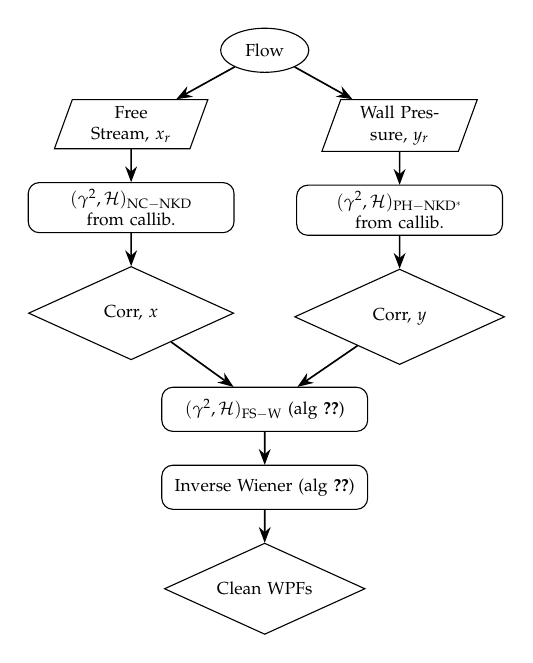
\begin{tikzpicture}[scale=0.7, transform shape, node distance=6mm and 18mm,
                    every node/.style={font=\small}]
        \centering
    % Start
        \node (start) [terminator] {Flow};

        % Two separate measurement boxes
        \node (refraw)   [meas, below left = 6mm and 14mm of start, anchor=north east]
            {Free Stream, $x_r$};
            
        \node (tretraw) [meas, below right = 6mm and 14mm of start, anchor=north west]
            {Wall Pressure, $y_r$};

        \node (Href) [proc, below=of refraw]
            {$ (\gamma^2,\mathcal{H})_{\mathrm{NC-NKD}} $ from callib.};

        \node (ref) [decision, below=of Href]
            {Corr, $x$};


        \node (Htret)  [proc, below=of tretraw]
            {$ (\gamma^2,\mathcal{H})_{\mathrm{PH-NKD^*}} $ from callib.};

        \node (tret)  [decision, below=of Htret]
            {Corr, $y$};

        \node (Hcomb)  [proc, below=57mm of start]
            {$ (\gamma^2,\mathcal{H})_{\mathrm{FS-W}} $ (alg~\ref{alg:H})};

        \node (corr)  [proc, below=of Hcomb]
            {Inverse Wiener (alg~\ref{alg:inv})};

        \node (post)  [decision, below=of corr]
            {Clean WPFs};

        \draw [line] (start) -- (refraw);
        \draw [line] (refraw) -- (Href);
        \draw [line] (Href) -- (ref);
        \draw [line] (start) -- (tretraw);
        \draw [line] (tretraw) -- (Htret);
        \draw [line] (Htret) -- (tret);
        \draw [line] (tret) -- (Hcomb);
        \draw [line] (ref) -- (Hcomb);
        \draw [line] (Hcomb) -- (corr);
        \draw [line] (corr) -- (post);

    \end{tikzpicture}
    \caption{Complete pressure processing pipeline for measurement of the WPFs through a pinhole microphone.}
    \end{figure}
\end{frame}

%--- Title page
% \begin{frame}
%     \setcounter{framenumber}{0}
%     \titlepage
%     \vfill
%     {\scriptsize \centering Thanks to DARPA for funding this work.\par}
% \end{frame}

% \begin{frame}

%     \begin{itemize}
%     %     \item Fix $U_e=14[\mathrm{m/s}]$
%         \item $\delta\approx 0.035[\mathrm{m}]$, $U_e \approx14[\mathrm{m/s}]$
%     \end{itemize}
%     \begin{table}[]
%         \centering
%         \begin{tabular}{lccccc}
%         \toprule
%         Pressure (psig) & 0  &  50 & 100 \\
%         \midrule
%         $u_\tau$[m/s] & 0.537 & 0.522 & 0.506 \\
%         $\nu/u_\tau$ [m] & 28$\times 10^{-6}$ & 6.6$\times 10^{-6}$ & 3.8$\times 10^{-6}$ \\
%         $\nu$ [m$^2$/s] & 14.9$\times 10^{-6}$ & 3.42$\times 10^{-6}$ & 1.93$\times 10^{-6}$ \\
%         $Re_\tau$ & 1 263 & 5 340 & 9 178 \\
%         \textcolor{blue}{ROI: $f$ [Hz]} & \textcolor{blue}{100--1 000} & \textcolor{blue}{100--1 000} & \textcolor{blue}{100--1 000} \\
%         \textcolor{blue}{ROI: $T^+$} & \textcolor{blue}{200--20} & \textcolor{blue}{800--80} & \textcolor{blue}{1 300--130} \\
%         \bottomrule
%         \end{tabular}
%     \end{table}

% \end{frame}

% \begin{frame}
%   \frametitle{Pinhole diameters}
%   \begin{figure}
%     \centering
%     \includegraphics[width=0.7\textwidth]{pinholes.pdf}
%   \end{figure}

%   \begin{itemize}
%     \centering
%         \item Testing pinhole diameters of $d=$ 2300, 700, 400 $\mu$m
%         \item Corresponds to $d^+ \approx$ 85, 93, 108
%         \item Under the frozen turbulence assumption, these sit around $T^+\sim 10$
%     \end{itemize}
% \end{frame}

\begin{frame}
  \frametitle{TF eq.}
  \centering
  \begin{align*}
    X(f;p_{\textrm{static}}) = \mathcal{F}\{p_{PH}(t;p_{\textrm{static}})\} \quad&\quad Y(f;p_{\textrm{static}}) = \mathcal{F}\{p_{NC}(t;p_{\textrm{static}})\}\\
    H(f;p_{\textrm{static}}) &= XY^*/(YY^*) \\
    \end{align*}
    \centering
  \begin{align*}
    Z(f;p_{\textrm{static}}) = \mathcal{F}\{p_{NKD}(t;p_{\textrm{static}})\} \quad&\quad Y(f;p_{\textrm{static}}) = \mathcal{F}\{p_{NC}(t;p_{\textrm{static}})\}\\
    H(f;p_{\textrm{static}}) &= YZ^*/(ZZ^*) \\
    \end{align*}
\end{frame}



\begin{frame}
  \frametitle{PH-NC}
  \begin{figure}
      \centering
      \includegraphics[width=0.9\textwidth]{final/tfs.png}
  \end{figure}
\end{frame}

\begin{frame}
  \frametitle{NC-NKD}
  \begin{figure}
      \centering
      \includegraphics[width=0.9\textwidth]{final/tfs_nc_nkd.png}
  \end{figure}
\end{frame}

\begin{frame}
  \frametitle{Spectra $u_{\tau}$ error}
  \begin{figure}
      \centering
      \includegraphics[width=0.9\textwidth]{final/tf_corrected_spectra_roi.png}
  \end{figure}
\end{frame}

\begin{frame}
  \frametitle{Spectra $p_{\textrm{static}}$ sensitivity}
  \begin{figure}
      \centering
      \includegraphics[width=0.9\textwidth]{final/tf_corrected_spectra_p_sensitivity.png}
  \end{figure}
\end{frame}

% ===============================
% --- Frame 1: Cross-spectrum (CSD)
% ===============================
\begin{frame}
  \frametitle{Cross-spectrum (CSD)}
  \centering
  \begin{align*}
    \Phi_{12}(f)
    &= \left\langle X_1(f)\,X_2^*(f) \right\rangle , \\[4pt]
    f\,\phi_{12}^+
    &= 
    f\,\frac{|\Phi_{12}(f)|}{(\rho\,u_\tau^2)^2} .
  \end{align*}
\end{frame}

\begin{frame}
  \frametitle{CSD}
  \begin{figure}
      \centering
      \includegraphics[width=0.9\textwidth]{CSDs/CSD.png}
  \end{figure}
\end{frame}

% ===============================
% --- Frame 2: Quad-spectrum (fourth-order cumulant)
% ===============================
\begin{frame}
  \frametitle{Quad-spectrum (fourth-order cumulant)}
  \centering
  \begin{align*}
    C_4^{(c)}(f)
    &= 
    \big\langle X_1(f)\,X_1(f)\,X_2^*(f)\,X_2^*(f) \big\rangle
    - \Phi_{11}(f)\,\Phi_{22}(f)
    - \Phi_{12}(f)\,\Phi_{12}(f), \\[4pt]
    f\,\phi_{12}^{(4)+}
    &=
    f\,\frac{|C_4^{(c)}(f)|}{(\rho\,u_\tau^2)^4} .
  \end{align*}
\end{frame}

\begin{frame}
  \frametitle{Quad-spectrum}
  \begin{figure}
      \centering
      \includegraphics[width=0.9\textwidth]{CSDs/quad.png}
  \end{figure}
\end{frame}

% ===============================
% --- Frame 3: Bispectrum and Bicoherence
% ===============================
\begin{frame}
  \frametitle{Bispectrum and Bicoherence}
  \centering
  \begin{align*}
    B_{xyz}(f_1,f_2)
    &= 
    \big\langle
    X(f_1)\,Y(f_2)\,Z^*(f_1{+}f_2)
    \big\rangle , \\[4pt]
    f_1 f_2\,|B|^+
    &=
    f_1 f_2\,\frac{|B_{xyz}(f_1,f_2)|}{(\rho\,u_\tau^2)^3} , \\[8pt]
    b^2(f_1,f_2)
    &=
    \frac{
    \big|\langle X(f_1)\,Y(f_2)\,Z^*(f_1{+}f_2)\rangle\big|^2
    }{
    \langle |X(f_1)Y(f_2)|^2\rangle\;
    \langle |Z(f_1{+}f_2)|^2\rangle
    } .
  \end{align*}
\end{frame}

\begin{frame}
  \frametitle{Bispectrum magnitude}
  \begin{figure}
      \centering
      \includegraphics[width=0.9\textwidth]{CSDs/bispec_mag_0psig.png}
  \end{figure}
\end{frame}

\begin{frame}
  \frametitle{Bispectrum magnitude}
  \begin{figure}
      \centering
      \includegraphics[width=0.9\textwidth]{CSDs/bispec_mag_50psig.png}
  \end{figure}
\end{frame}

\begin{frame}
  \frametitle{Bispectrum magnitude}
  \begin{figure}
      \centering
      \includegraphics[width=0.9\textwidth]{CSDs/bispec_mag_100psig.png}
  \end{figure}
\end{frame}

\begin{frame}
  \frametitle{Bicoherence}
  \begin{figure}
      \centering
      \includegraphics[width=0.9\textwidth]{CSDs/bispec_bicoherence_0psig.png}
  \end{figure}
\end{frame}

\begin{frame}
  \frametitle{Bicoherence}
  \begin{figure}
      \centering
      \includegraphics[width=0.9\textwidth]{CSDs/bispec_bicoherence_50psig.png}
  \end{figure}
\end{frame}

\begin{frame}
  \frametitle{Bicoherence}
  \begin{figure}
      \centering
      \includegraphics[width=0.9\textwidth]{CSDs/bispec_bicoherence_100psig.png}
  \end{figure}
\end{frame}










\end{document}
